\exerciseset{A weight of 100lb is suspended from two chains, making angles with the vertical of $\theta$ and $\varphi$ as shown in the figure below.
\begin{center}
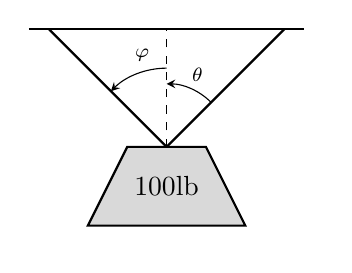
\begin{tikzpicture}
    \filldraw[thick,black,fill=gray!30] (-.5,0) -- (.5,0) -- (1,-1) -- (-1,-1)--cycle;
    \draw (0,-.5) node {100lb};
    \draw [thick] (-1.75,1.5) -- (1.75,1.5);
    \clip (-1.5,1.5) rectangle (2,-1.25);
    \draw [thick,rotate=135] (0,0) -- (3,0);
    \draw [thick,rotate=45] (0,0) -- (3,0);
    \draw [dashed] (0,0) -- (0,2);
    \draw [rotate=45,->,>=stealth] (.8,0) arc (0:45:.8);
    \draw [rotate=67] (1,0) node {\scriptsize $\theta$};
    \draw [rotate=90,->,>=stealth] (1,0) arc (0:45:1);
    \draw [rotate=105] (1.2,0) node {\scriptsize $\varphi$};
\end{tikzpicture}
\end{center}
In Exercises}{,  angles $\theta$ and $\varphi$ are given. Find the force applied to each chain.}{

\exercise{$\theta = 30^\circ$,\quad $\varphi=30^\circ$}{The force on each chain is  $100/\sqrt{3}\approx 57.735$lb.}

\exercise{$\theta = 60^\circ$,\quad $\varphi=60^\circ$}{The force on each chain is  $100$lb.}

\exercise{$\theta = 20^\circ$,\quad $\varphi=15^\circ$}{The force on the chain with angle $\theta$ is approx. $45.124$lb; the force on the chain with angle $\varphi$ is approx. $59.629$lb.}

\exercise{$\theta = 0^\circ$,\quad $\varphi=0^\circ$}{The force on each chain is 50lb.}

}
